\chapter{Discussion and Conclusions}

In this thesis is explained a novel form of generating trans-genetic circuits.  Using ParAlleL, a full adder and a full subtractor were achieved including a digital-like display showing numbers from 0 to seven once the proper 3-bit inputs were added into the system. Here each input bit is considered in two forms, ZERO or ONE, each of which is essential to certain output agents, any arbitrary pattern of outputs for any pattern of inputs can be generated, making all kinds of binary operation possible. The ability of this system to solve information-related and decision-making problems gets it close to the Alan Turing’s theoretical machine.  Biological implementation, rather than electronical processes, adds their own challenges but also follow the same Boolean system where an input enters the system to be later analysed via an algorithm that is in turn processed in a computationally prepared cell or population, following Boolean logics, to finally generate an output that can be detected, reprocessed, or discontinued. Nature could even have processes that computes function not even computable on a Turing machine, helping us to perform new computations overhauling the definition of computability \citep{grozinger2019pathways}. 

\begin{figure}[!ht]
  \centering
  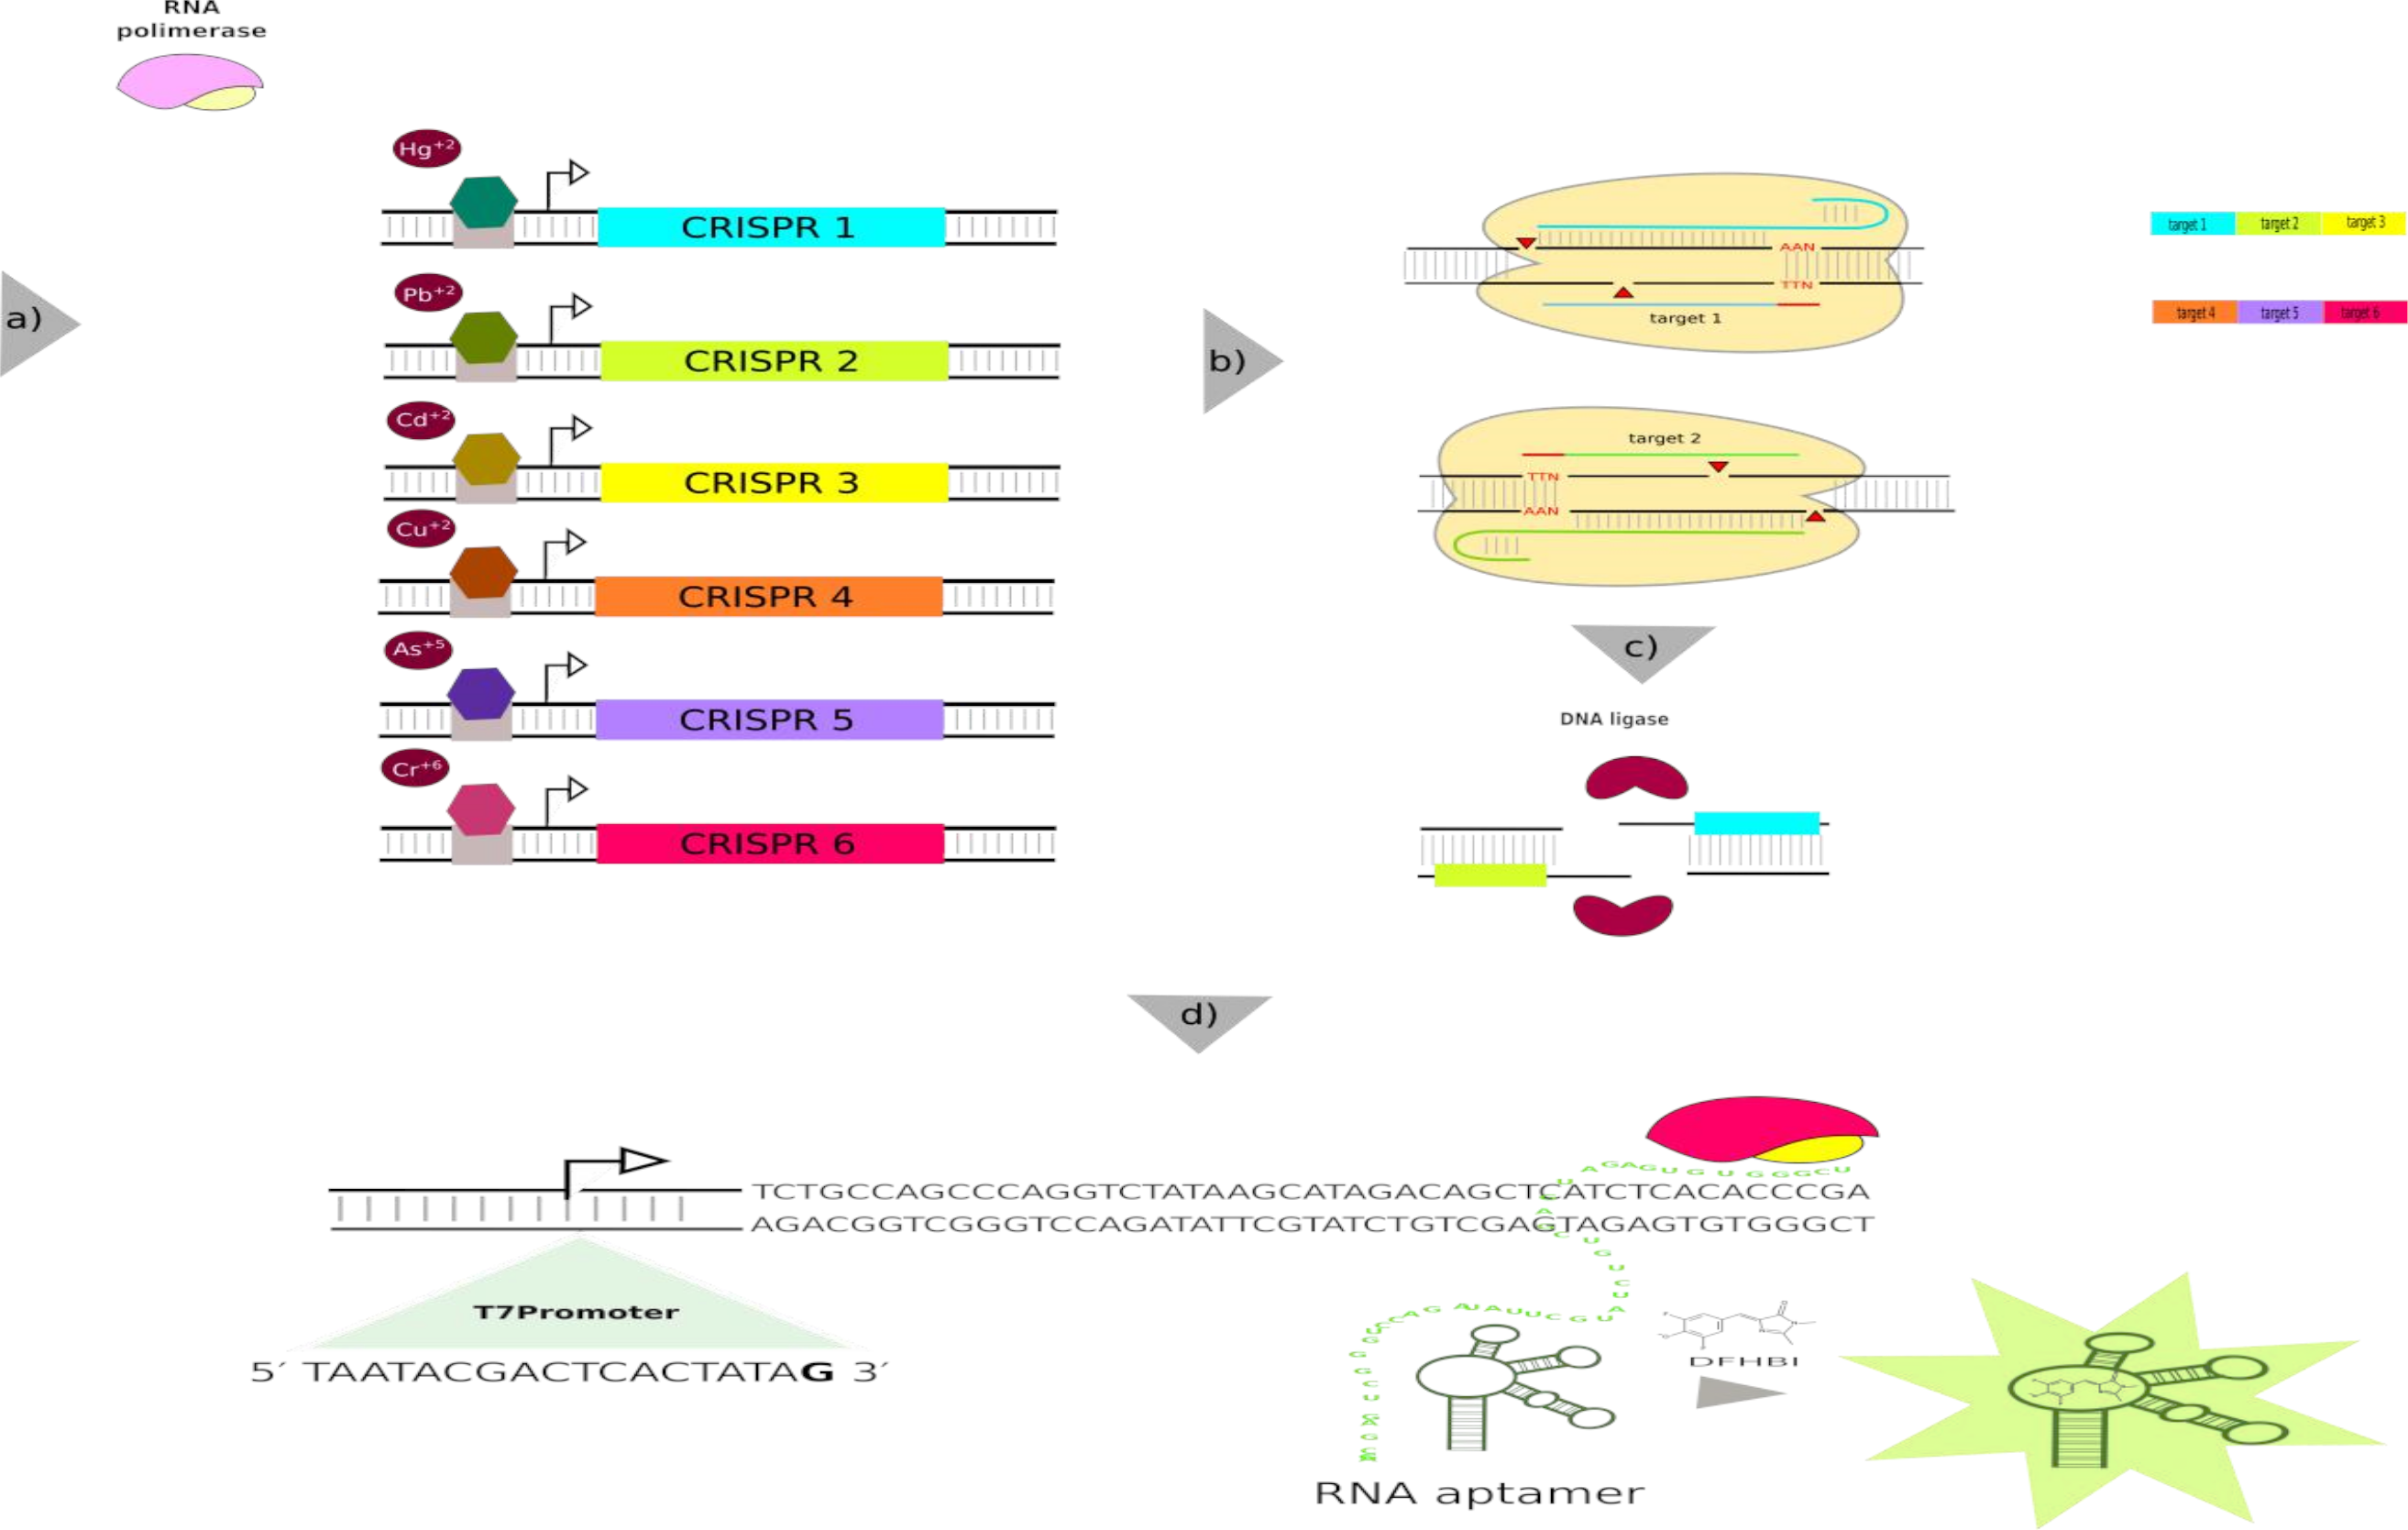
\includegraphics[width=1\textwidth]{discussion/chapter/figs/dnalogic.png}
  \caption{Proposed DNALogic system. A) crRNA expression is regulated by inducible promoters B) Ribonucleoprotein formation is followed by recognition and cutting of the target DNA C) Ligation of the overhangs produced by the Ribonucleoprotein generates a transcriptional unit D) Expression of the transcriptional unit generates a functional fluorescent RNA aptamer.}
  \label{fig.discu1}
\end{figure}

Even though here we use a population of living cells, these could be replaced by a totally in vitro reaction where a transcriptional-only genetic network can be used, without further need of translation. Each agent in this case, rather than a cell, can be a plasmid or a double stranded DNA that does not possess functional transcriptional networks. As cell-free systems can assemble DNA parts in vitro at very low cost by using cell extracts instead of enzyme cocktails \citep{casini2014one} and Golden Gate Assembly is an excellent tool to assemble multiple DNA fragments in a defined linear order, by using type IIS restriction enzymes \citep{engler2008one} , these techniques may be combined to generate a new and inexpensive in vitro system, which through DNA assembly and processing (hereafter DNALogic) would be able to sidestep common problems associated with the use of live cell based systems. As a "triggering" step is vital for the DNALogic processing machinery, the novel CRISPR/Cpf1 technology (or similar) could be used to generate the respective recognition and cutting steps. CRISPR/Cpf1 generates 5' overhanging cuts, producing 8 nt sticky ends and cleaving at the 14th base from the PAM site TTN \citep{Lei2017a, li2016c}. Due to its similarities to Type IIS restriction enzymes, Cpf1 or any simile enzyme can be used to generate a new kind of Golden Gate Assembly, which would not rely on the presence or absence of cutting sites, but on gRNA. The gRNA expression system can be combined with the recognition step, working as a transduction system between the detection and processing steps. This CRISPR triggered sequence recognition, followed by cutting and ligation steps, would result not only in a fully functional transcriptional unit, but also in a different double stranded genetic sequence, complying with the parameters for synthetic memory proposed and demonstrated in vivo by \citet{siuti2013synthetic}. This would create DNA memory that can not only be later amplified and processed by sequencing and/or PCR (late response), but also generating RNA expression of a fluorescent aptamer or a further gRNA if there would be formation of a proper transcriptional unit (immediate response). Proposed mechanisms can be seen on Figure \ref{fig.discu1}. 
RNA aptamers also suffer from several limitations as incorrect folding is observed under non optimal thermal or ionic conditions \citep{autour2016ispinach}. Even though improved aptamers with a stronger secondary structure, such as Broccoli and iSpinach, show increased stability under non-optimal conditions \citep{filonov2014broccoli, autour2016ispinach}, both aptamers are based in the 95 base core sequence of Spinach2 which need to be flanked by a tRNA scaffold, to increase the stability of their secondary structures \citep{filonov2014broccoli, autour2016ispinach, strack2013superfolding}. However, most of them were designed for in vivo usage (e.g. analysing RNA quantities) and have not been tested as outputs for a cell-free sensor besides this work and the one from \citet{jung2020cell}. Such a sensor could require only transcription, not translation, thus being faster and simpler.

Cell-free systems (CFS) are not without their limitations; since their very nature is to be a defined, precisely controlled system that lacks self-replicating functionality, they depend on a limited quantity of supplies, such as ATP, amino acids, and nucleotides \citep{kwon2015high}. Even though the coupling of transcription and translation accelerates the product formation, proteins still need to acquire their secondary, tertiary or even quaternary conformation to become functional, even sometimes needing post-translational modifications to work. 

Consequently, in-vitro synthesis of protein is limited by two dimensions: the overall maximum protein amount that can be synthesized with the supplied components, and the time during which the CFS stays active before background processes and chemical deterioration have used up supplies or inactivated the system \citep{carlson2012cell, bernhard2013cell,kwon2015high}. One of the most promising applications of CFS is the possibility of designing cell-free biosensors, which do not present a living prospect subject to the current GMO legal regulations and offer an alternative to standard analytical techniques, such as ICP-MS and ICP-OES. However, cell-free biosensors that rely on protein expression also present the common limitations of CFS, such as a long response time and a lack of precursor regeneration. Sensors that could function without the need for protein expression would drastically reduce the requirements for such a system.
\begin{figure}[!ht]
  \centering
  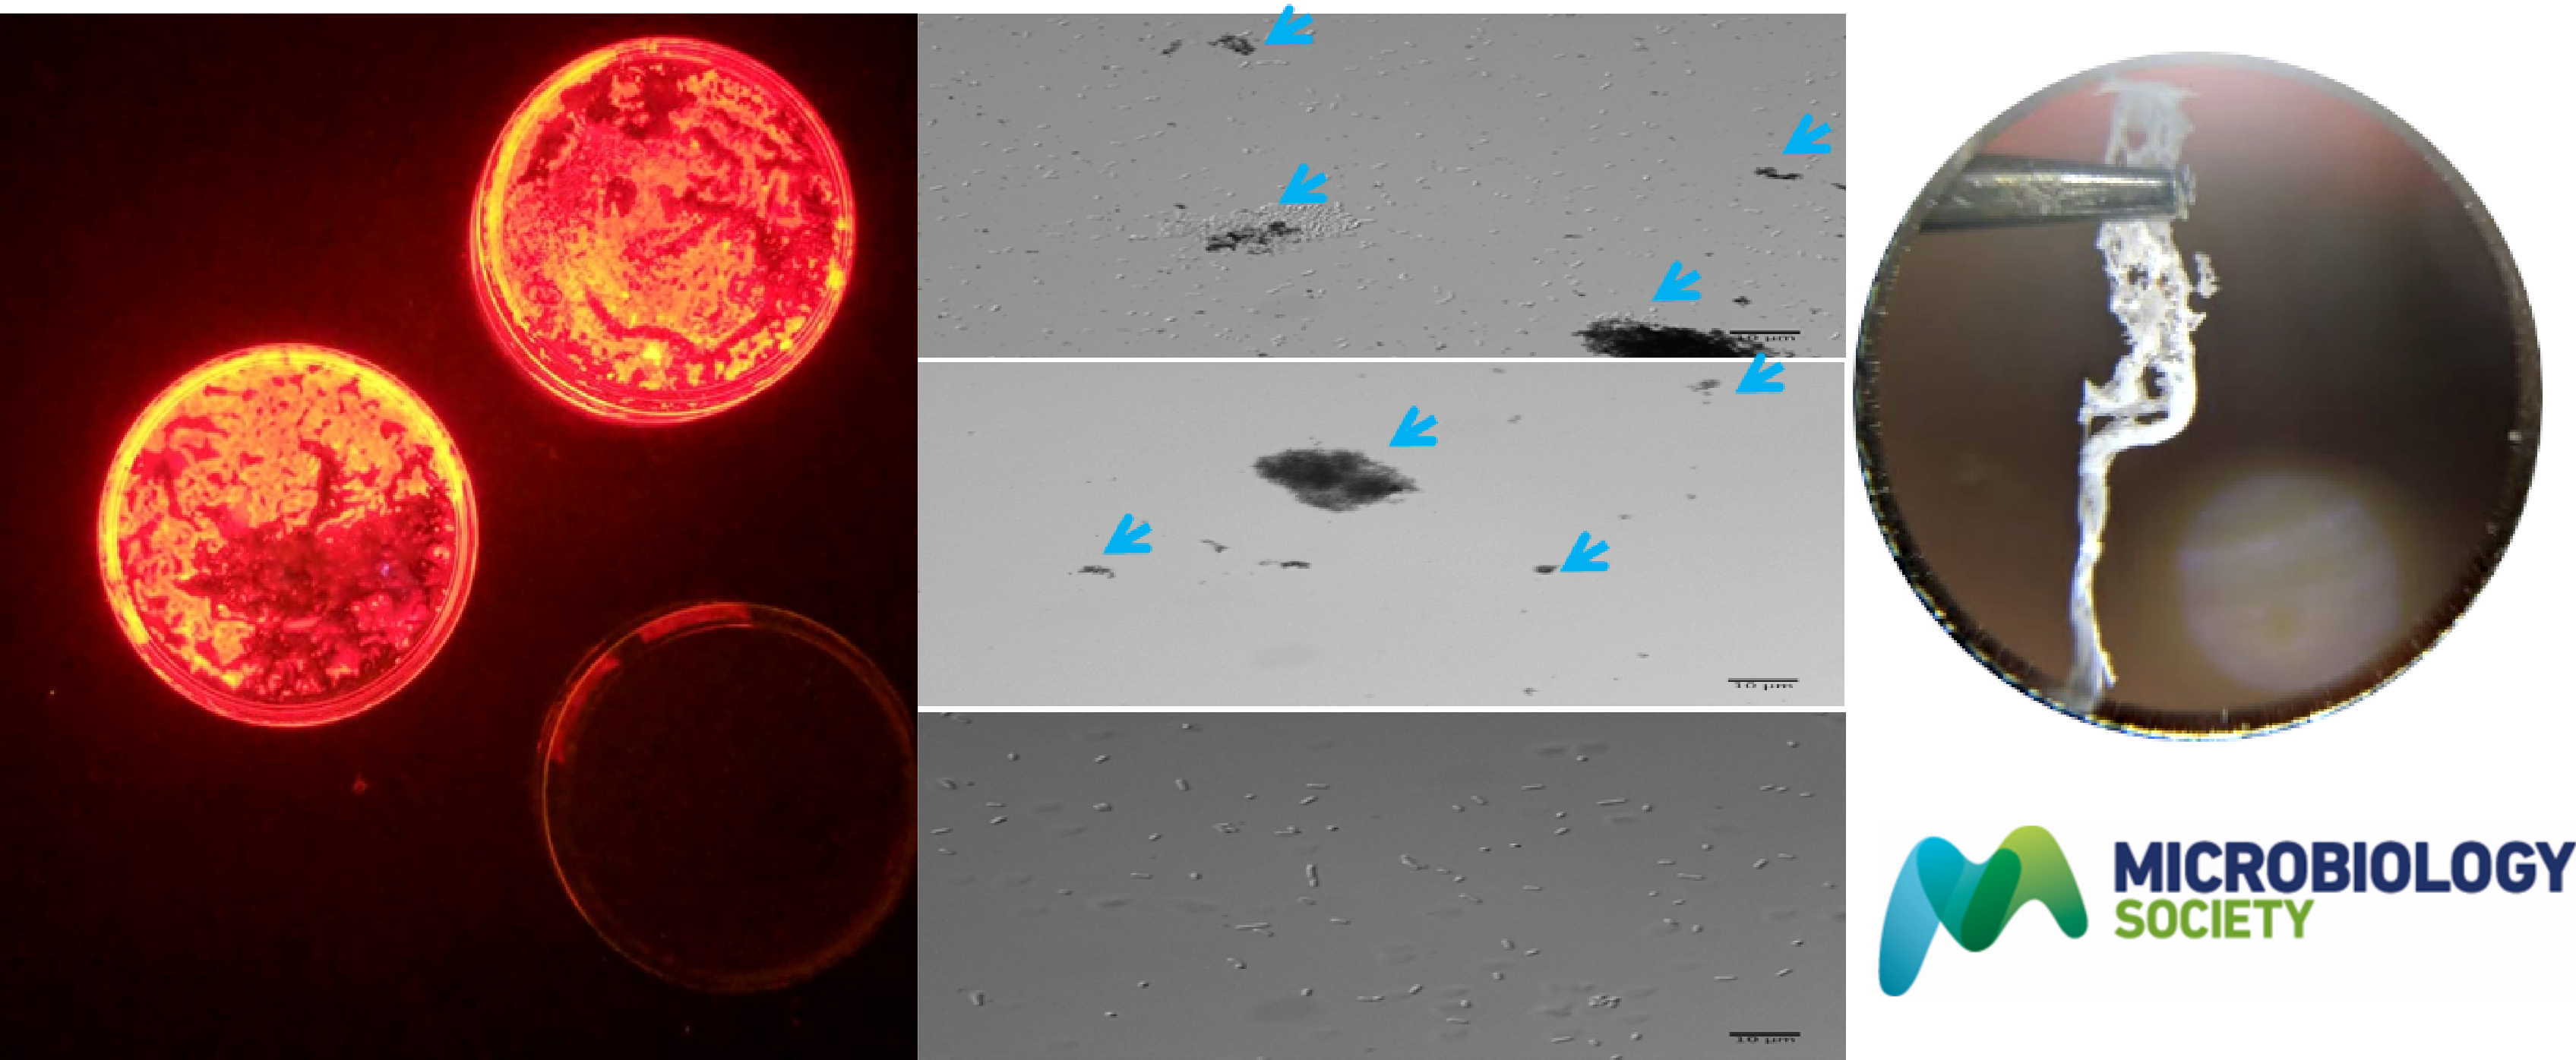
\includegraphics[width=0.9\textwidth]{discussion/chapter/figs/bioplastics.png}
  \caption{PHB Production Using Cell-Free Systems. Left. Bioplastic detection under blue light after Nile Red staining. Middle. in vivo and in vitro PHB production. Right. Bioplastic produced and purified from CH34 cultures. Work sponsored by the Microbiology Society and performed with the help of Nuoya Chen}
  \label{fig.discu2}
\end{figure}

\cite{moore2017cell} have attempted to solve this issue by using non-model bacteria, such as \textit{Bacillus} or \textit{Streptomyces}, for the generation of new cell-free TX/TL systems. This approach can be applied to other organisms, such as extremophiles, in order to use their unique capacities. For example, in this thesis is used the non-model bacteria \textit{Cupriavidus metallidurans} which possesses the capability to tolerate, remove and degrade diverse environmental pollutants \citep{millacura2017degradation}. This cell-free extract is simple to prepare by using a low-salt buffer and shows increased tolerance for heavy metals making it possibly superior to others as a heavy metal sensor. Preliminary results show that the anabolic and catabolic capabilities of this cell extract are conserved after lysis, here demonstrated via bioplastic production (Figure \ref{fig.discu2})  and by catechol degradation via catechol-1,2-dyoxygenases and catechol-2,3-dyoxygenases (Figure \ref{fig.discu3}) respectively. Even though further development is required, this novel cell-free chassis could become a standard for mass production considering versatility and robustness showed once compared with \textit{E. coli} based ones.

\begin{figure}[!ht]
  \centering
  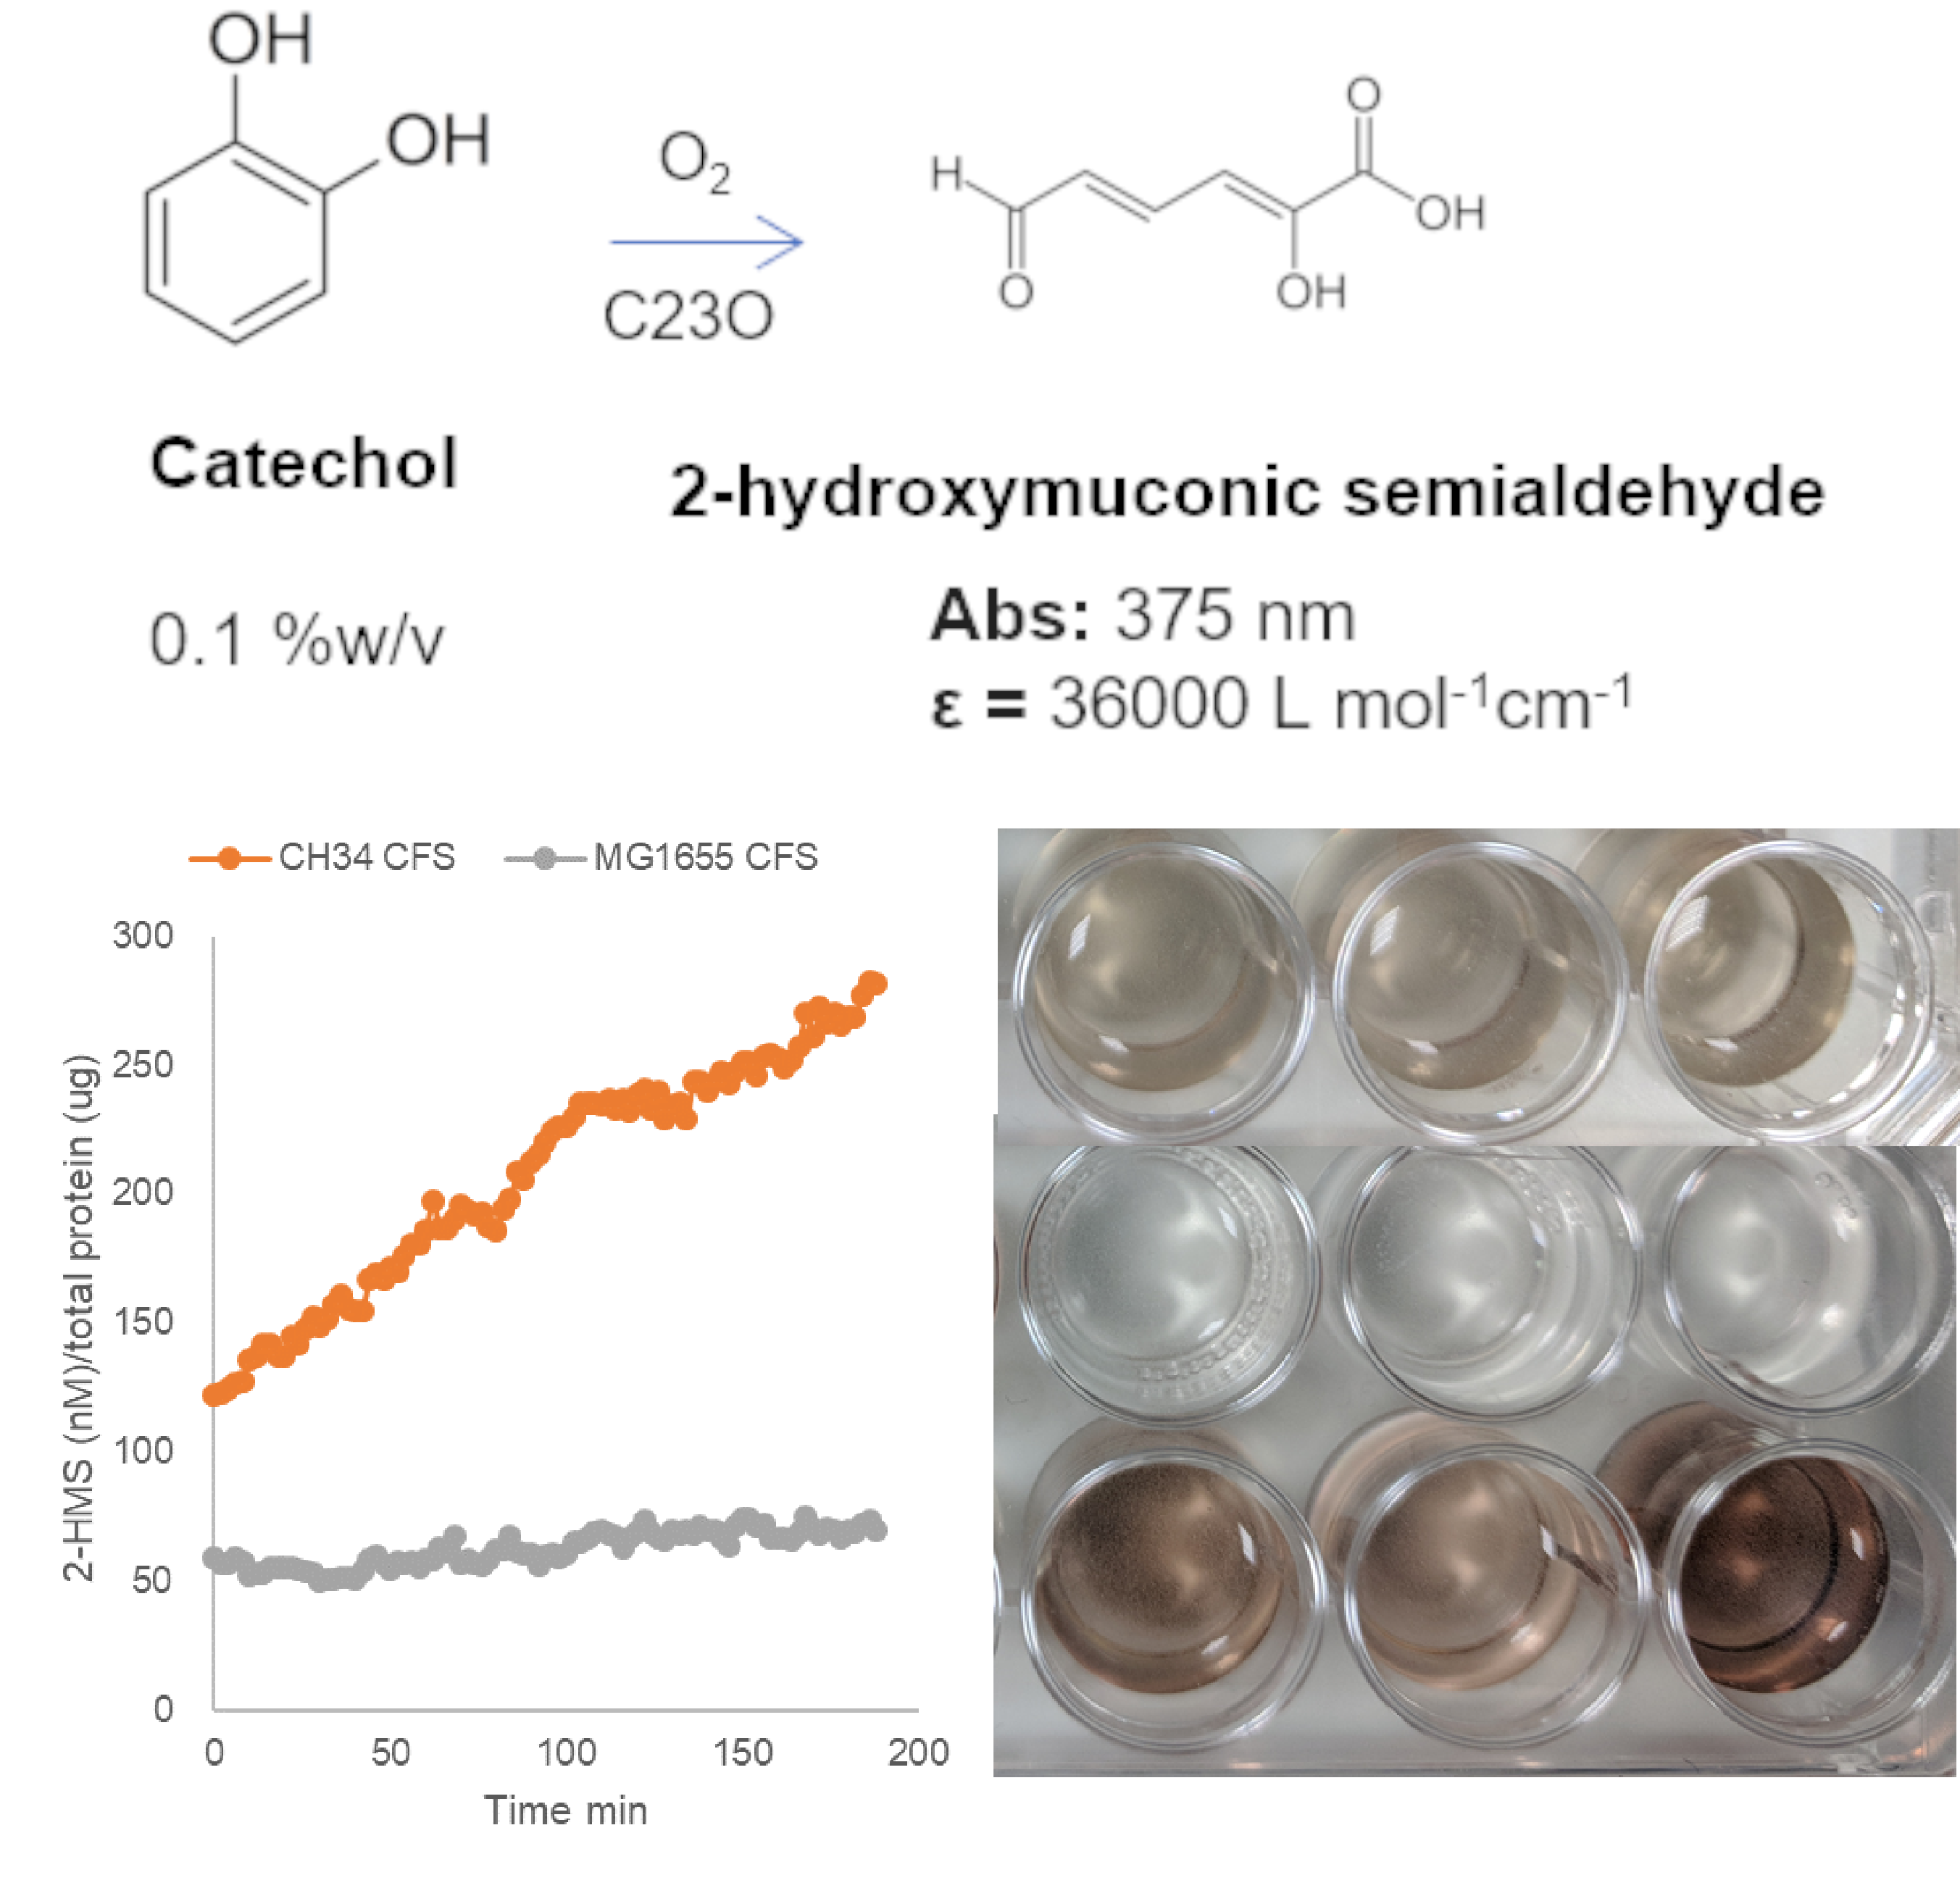
\includegraphics[width=0.7\textwidth]{discussion/chapter/figs/degradation.png}
  \caption{Catechol-2,3-dioxygenase activity assay using \textit{Cupriavidus} cell-free system. Upper. beta-cleavage of the catechol ring and formation of 2-hydroxymuconic semialdehyde. Bottom. \textit{Cupriavidus} cell-free catechol degradation.}
  \label{fig.discu3}
\end{figure}


Another challenge for CFS is to analyse multiple variables simultaneously. As they rely on the normal cell processing/synthesis machinery (interaction between transcription factors, polymerases, ribosomes, and other diverse macromolecules), they suffer the same issues as a living organism. Furthermore, when complex interactions are carried out, problems may arise due to kinetic mismatches, lack of oscillation or Boolean/Reversible designs \citep{guz2016bioelectronic}. The generation of cell-free systems that respond to variables using totally synthetic processing machinery seems to be one of the most promising approaches. There have been some attempts to generate logic gates without mimicking normal cell machinery \citep{bordoy2016transcriptional, chatterjee2016computing, kim2011switch, zhang2016dna}, however, due to their dependence on translation and/or the need for manual addition of foreign oligonucleotides (Kim et al., 2014) they still show slow response. Additionally, some of them rely on recombination processes that make their implementation even more complicated than under \textit{in vivo} conditions \citep{zhang2016dna}. In electronics, a single circuit accepts one or more binary inputs to generate one or more binary outputs. There have been many attempts to replicate such circuits using in vivo genetic networks. A typical biological logic gate consists of an output macromolecule that is produced only if the corresponding pattern of inputs is present, inputs that are commonly associated with the presence of transcriptional regulators, transcription factors, polymerases or other macromolecules \citep{silva2008mining}.


Since scientific data in Synthetic Biology is massively increasing, novel analysis techniques than go further than standard human gathering need to be implemented. For instance, machine learning algorithms and artificial intelligence can be used to gather, process, and analyse scientific reports. An example is shown in Figure \ref{fig.discu4} were Natural Language Processing techniques were used to analyse the complete collection on Synthetic Biology publicly available on BioRxiv. There are hundreds of scientific research manuscripts published every year and information can get missing or hidden-in-plain-sight. Machine learning could grant the link between the words used in research articles and the data referenced on it, also it could allow prediction of new technologies to come by simply analysing both topics of high and low interest for the research community. With enough computational power massive quantities of data could be analysed even in real-time, crossing not only with official repositories but also social networks specialised in research or not.

\begin{figure}[!ht]
  \centering
  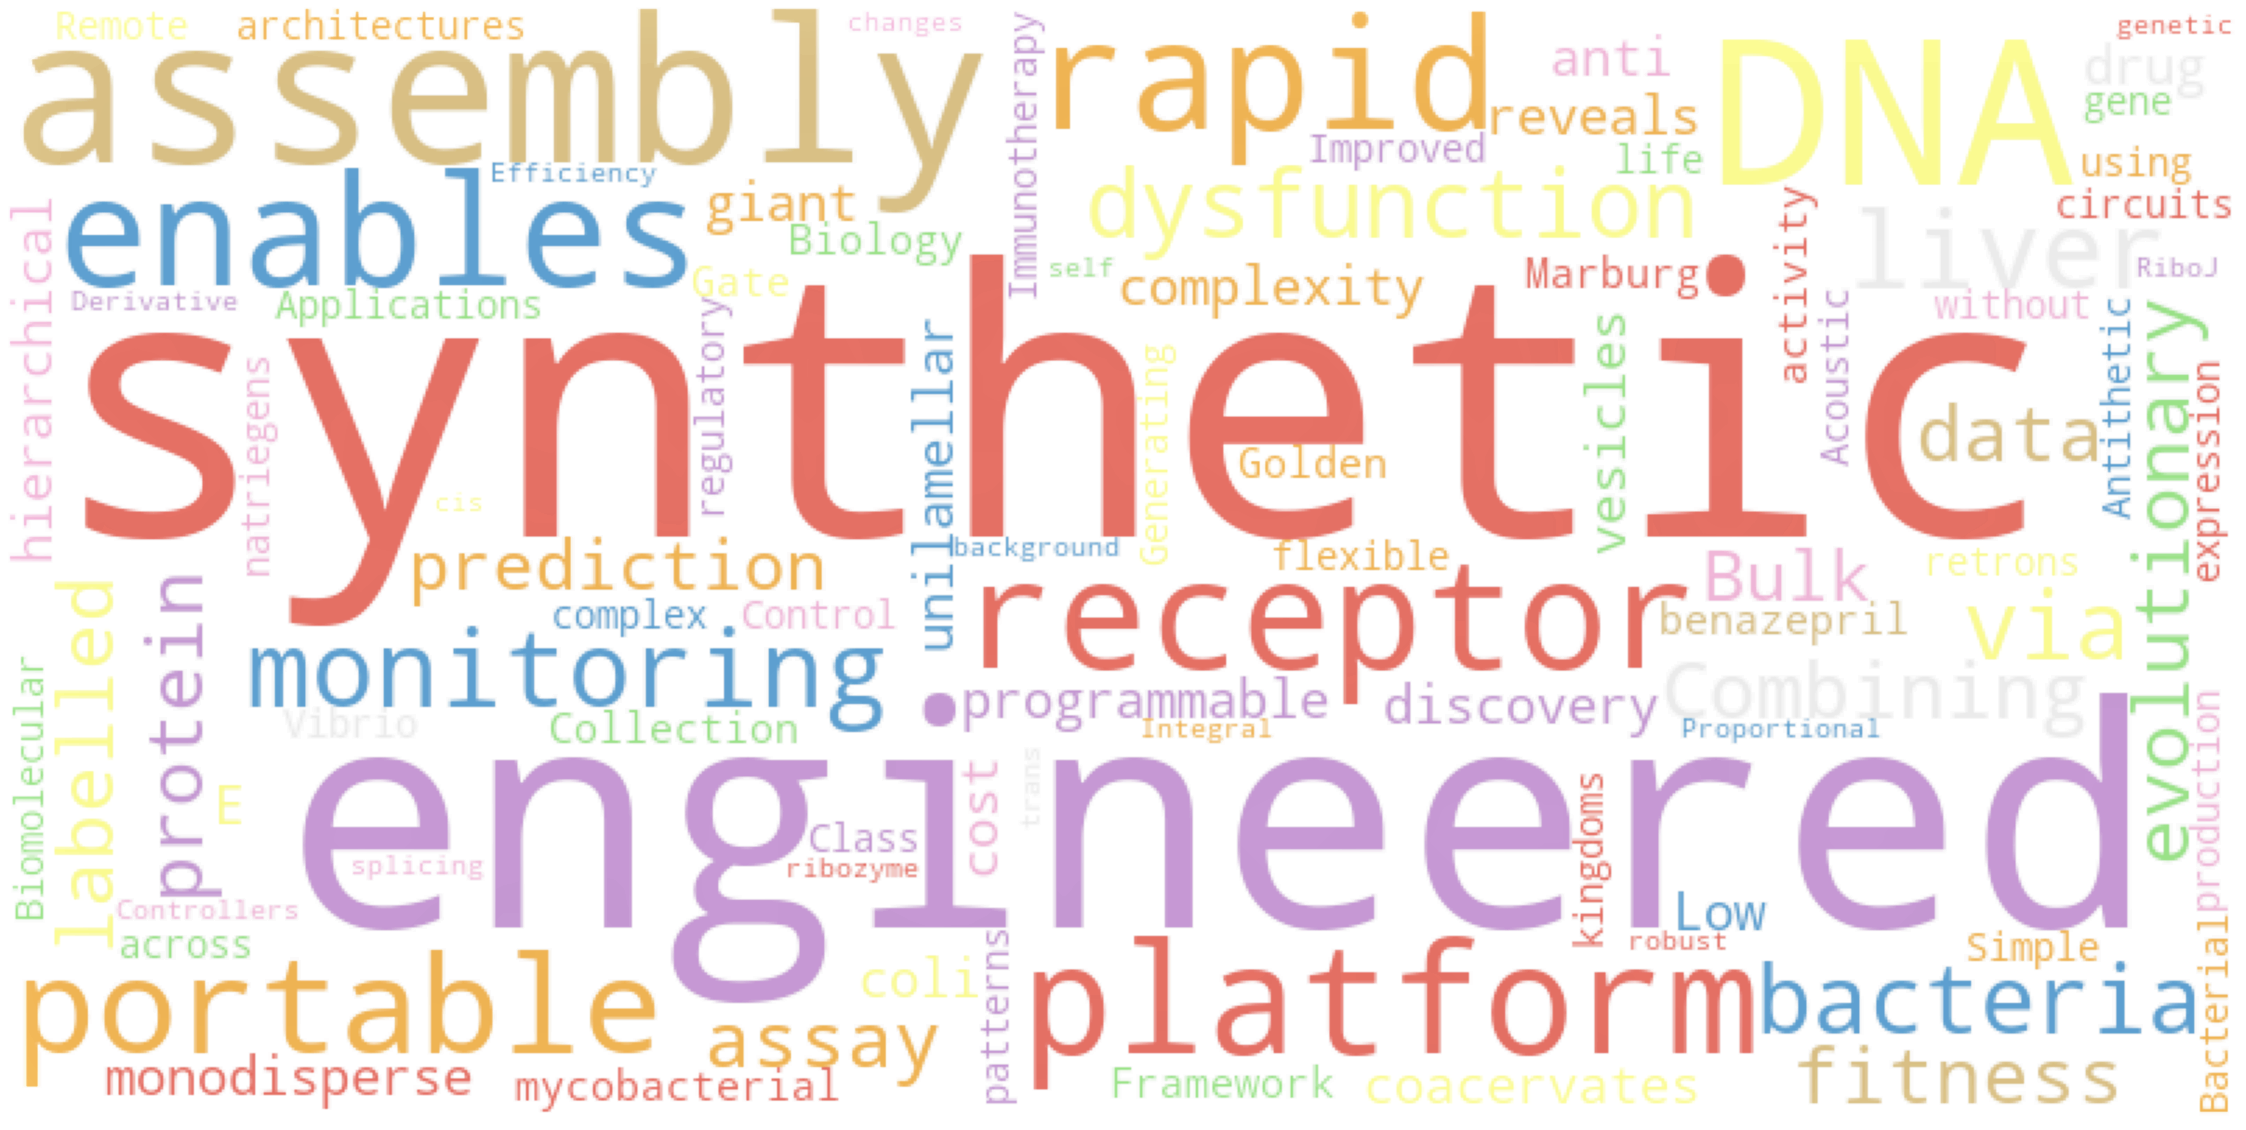
\includegraphics[width=0.9\textwidth]{discussion/chapter/figs/wordcloud.png}
  \caption{Natural Language Processing (NLP) analysis of BioRxiv's Synthetic Biology collection. Article titles from the entire BioRxiv synthetic biology collection were analysed using Natural Language processing (NLP) techniques. All 220 articles were collected via web scrapping and unnested into 2552 tokens and stopwords later removed. Most common 100 words are here plotted as a WordCloud. Full analysis available at https://gist.github.com/millacurafa/0151170cf971d1ae46092f32b4d7c2a2}
  \label{fig.discu4}
\end{figure}

Another interesting feature of current technologies would be the usage of machine and deep learning algorithms to analyse metagenomic or genomic analyses. Sequencing techniques are getting cheaper each time and since it has been proved than mutations can be generated during genetical engineering, rather than just analysing a few genes and phenotypes the scientific community could start preparing into massive genomic analyses. Assemblies could be simplified, together with SNPs and INDELs detection. Additionally, algorithms could be generated to generate inexistent sequences that would allow to go even further than what it is available in nature. For instance, the terms minimal absent words (MAWs), nullomers and primes all describe sequences that do not occur in the entire genome or proteome of an organism \citep{hampikian2007absent, koulouras2020significant}. Primes are the shortest sequences that are not found across all known species, whereas nullomers are the shortest possible absent motifs in a species, MAWs including both definitions. But what are the shortest or even largest sequences present in all organisms (aka popularly as the sequence of god). These still have theoretical significance as sequences that cannot exist on nature due to them causing death in organisms or simply because during natural selection were not prioritized. A world of new opportunities lay in sequences that are beyond nature and the scope of Synthetic Biology should be broaden in that direction allowing to solve the unsolvable.